\documentclass{article}
\usepackage{graphicx} % Required for inserting images
\usepackage{fancyhdr}
\pagestyle{fancy}

\title{final-assignment-project}
\author{mahdi td}
\date{Bahman 1402}

\begin{document}
\cfoot{\thepage}
\lhead{\thepage}
\maketitle
\newpage

\tableofcontents
\fancyhead[R]{\textbf{CONTENTS}}
\newpage
\fancyhead[R]{\textbf{Git and Exploration}}
\section{Git and GitHub}
\subsection{Repository Initialization and Commits}
At first I got into the github website opened my account and went into the repositories menu and created a new repository named finale-assignment-repo with having a readme file inside it.
\subsection{GitHub Actions for LaTeX Compilation}
I searched about linking up latex and git hub with github actions I made a few tags to check if its working properly.\\
for this linking i made a file with .github/workflows and copied the file was made in the class repository and pasted it on my file.\\
I've encountered many challenges and i got tired so much\\
any tag i made was checking on website and turning out to have an error in file.\\
i changed my files many times i changed names and paths to the files after some time i finally made it OK.\\
then i started writing the tex file in vscode and pushing it in the git.
\section{ Exploration Tasks}
\subsection{Vim Advanced Features}
\textbf{A.}  you can use ctrl+p or ctrl+n for filling a word that you used before on that page for example if you typed "hello world" before you can auto fill the "he" to "hello" by pressing ctrl+p or ctrl+n.\\
\textbf{B.}this feature is for opening files in vim.you can select a file path on your text and then press gf for opening the path through that file and if i understanded correctly you will create a file with that path and name if it does not already existing.\\
\textbf{C.}this feature is for opening Url's and if you select the url text and press gx you are opening the url in your default searching web like chrome or bing.\\
\subsection{Memory profiling}
\subsubsection{Memory Leak}
A memory leak is a type of programming error that occurs when a program fails to release memory that is no longer needed.\\for example we learned to use malloc or calloc functions in c programming these functions assign a space to our needed job in program and we should free them when they are no longer needed. if an error happens and they could not be free meemory.\\
these type of errors can lead to system inability.
\subsubsection{Memory profilers}
Valgrind is a powerful tool that can help detect memory leaks and other memory-related errors in C and C++ programs. Valgrind can detect memory leaks by identifying memory that has been allocated but not freed.\\To use Valgrind, you need to compile your program with debugging symbols and then run it under Valgrind’s control . Valgrind will report any memory leaks or other memory-related errors that it detects . Valgrind can also provide detailed information about the source of the memory leak, including the line of code that allocated the memory 
\subsection{GNU/Linux Bash Scripting}
\subsubsection{fzf}
Fuzzy searching is like a smart way of looking for things on a computer. Instead of needing things to be exactly the same, it's okay if there are a few mistakes, like misspelled words. So, even if you don't type everything perfectly, the computer can still find what you're looking for and show you results that are pretty close. It's like a helpful tool that understands that people might make small errors when searching for information.\\
when you run ls l fzf, it makes a list of files and directories in the current directory using ls, and then passes that list to fzf for searching and finding what you want in a different way.
\subsubsection{Using fzf to find your favorite PDF}
fd -e pdf\\
This command searches for files with the .pdf extension using the fd command.\\
fd -e pdf l fzf - -query="riazi1"\\
This command uses fd to find all files with the .pdf extension, and then pipes the result to fzf. The - -query="riazi1" option sets the initial search in fzf to "riazi1", allowing you to filter the list and quickly locate the PDF file you're interested in.
\subsubsection{Opening the file using Zathura}
zathura "\$(fd -e pdf l fzf - -query="riazi1")"\\
This command uses fd to find all PDF files, then pipes the result to fzf for interactive selection. The selected PDF file is then passed to the zathura command using command \$. Replace "riazi1" with the actual file you're looking for.
\section{Git and FOSS}
\subsection{Issues}
screen shots are included in next page.
\newpage
\fancyhead[R]{\textbf{screen shots}}
\begin{figure}
\begin{center}
    

    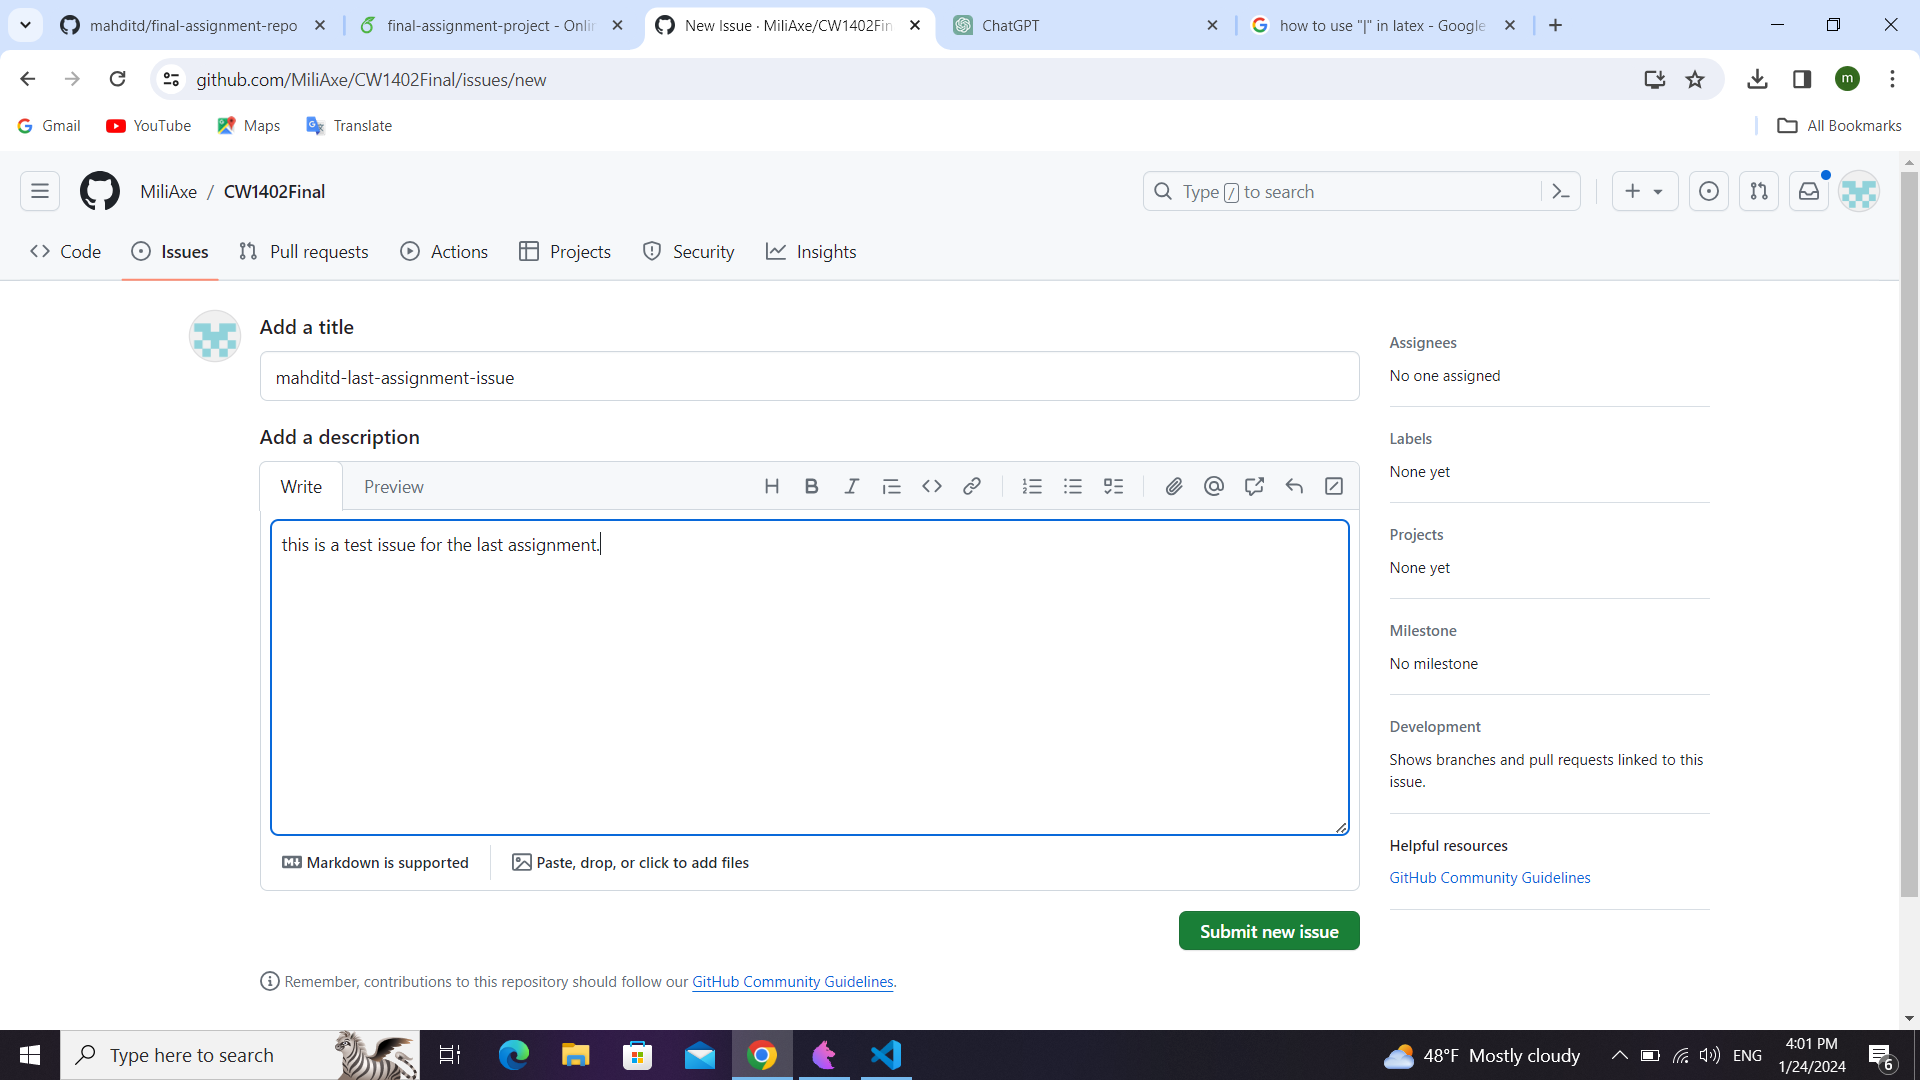
\includegraphics[width=0.8\linewidth]{Screenshot (32).png}
    \caption{issues first screenshot}
    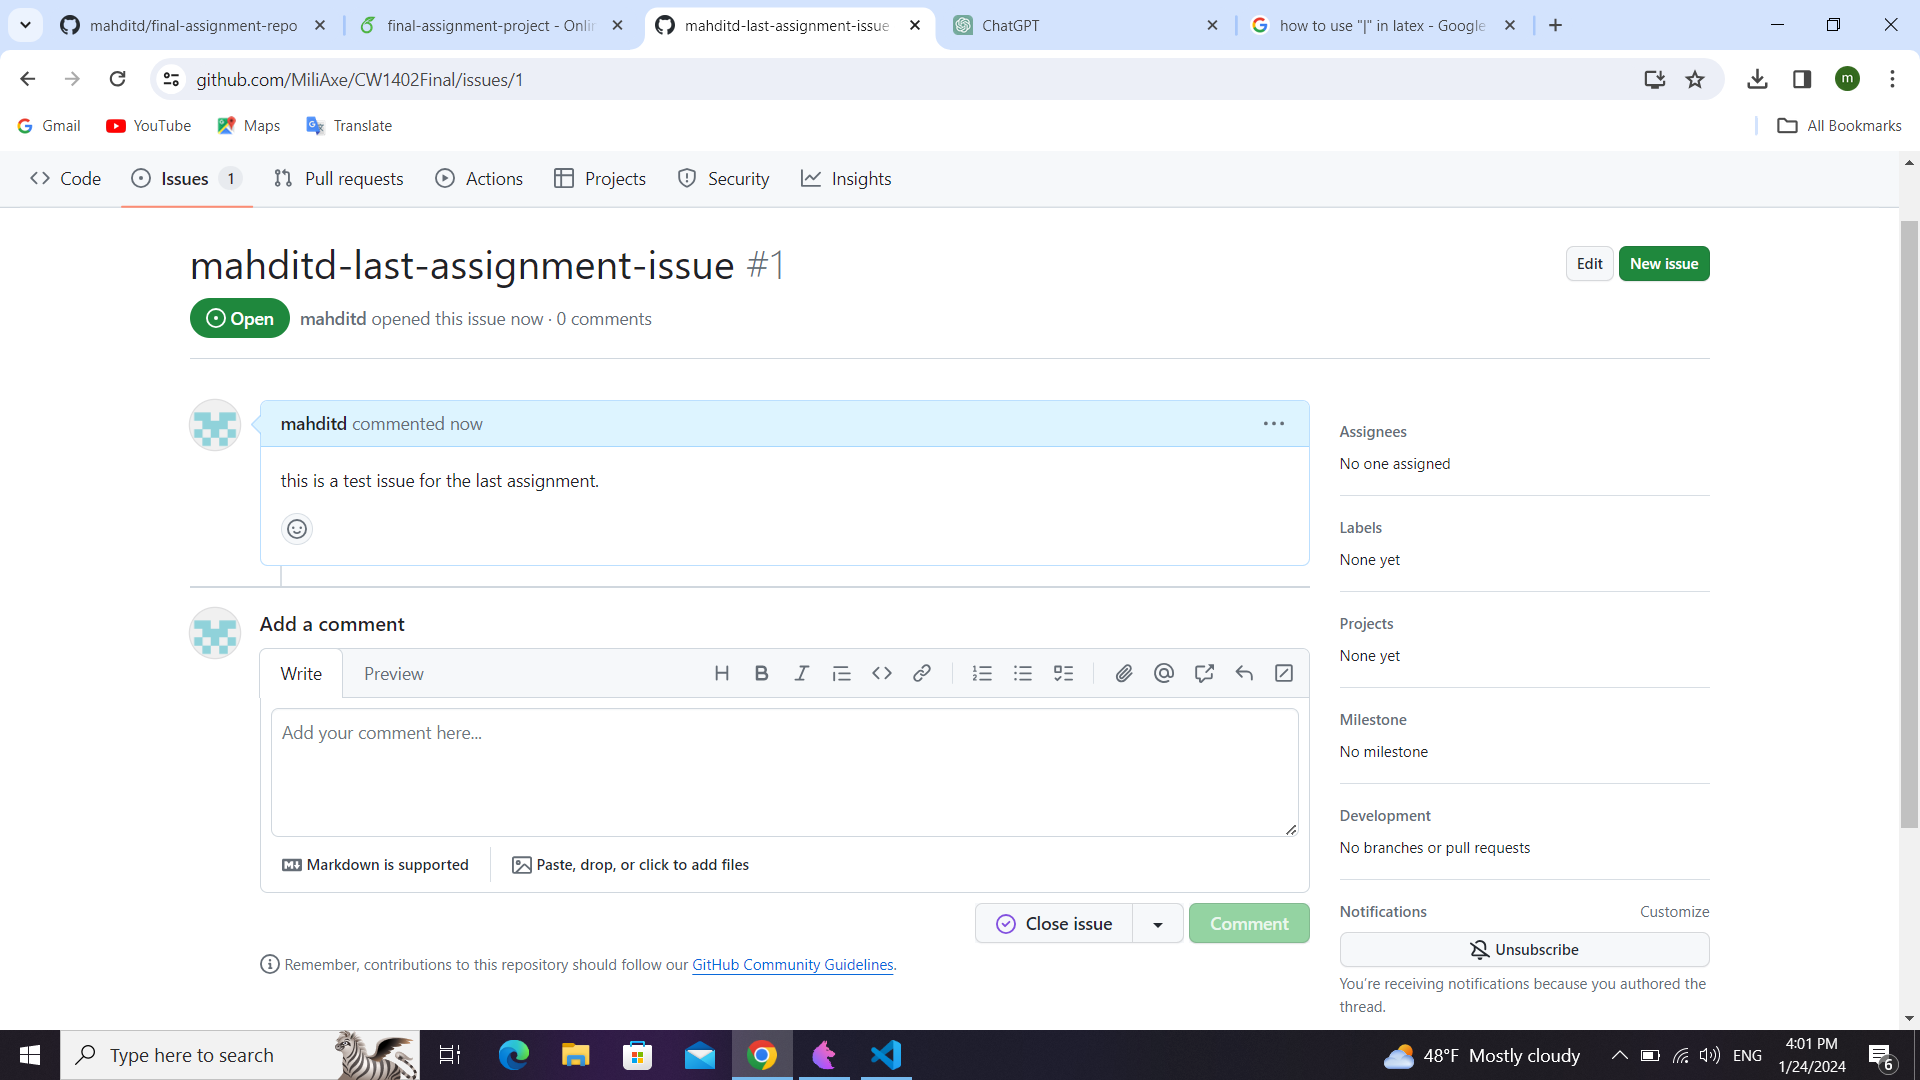
\includegraphics[width=0.8\linewidth]{Screenshot (33).png}
    \caption{issues second screenshot}
    \end{center}
\end{figure}







\end{document}
